\subsection{\gls{ros2}) \cite{noauthor_ros_nodate}}
\label{partie:ros}

\gls{ros} est un framework conçu pour le développement d'applications robotiques. Bien qu’il ne soit pas un système d’exploitation à proprement parler, il agit comme un middleware qui facilite la communication entre les sous-systèmes du robot (capteurs, actionneurs, estimation, contrôle, planification). Il fournit un ensemble d’outils, de bibliothèques qui simplifient la création de systèmes robotiques, le déploiement et le débogage. Sa force réside dans l’organisation et la standardisation des échanges d’informations entre composants, ce qui rend l’intégration de modules plus simple. \gls{ros} s’intègre également à des environnements tiers, par exemple via une ToolBox Matlab/Simulink, permettant d’utiliser \gls{ros} depuis Matlab/Simulink.

Dans l'architecture \gls{ros}, chaque programme autonome est appelé \textit{noeud}, et un ensemble de \textit{noeud} est appelé \textit{package}. La communication entre les noeuds se fait par l'échange de messages via des canaux appelés \textit{topics}, selon un modèle \textit{publisher-subscriber}. Un noeud \textit{publisher} envoie des données sur un topic, tandis qu'un noeud \textit{subscriber} les récupère. Lorsqu’ils sont connectés au même réseau, plusieurs appareils peuvent accéder aux mêmes topics. Cela facilite grandement la communication entre les différents noeuds, qu'ils soient sur le même appareil ou sur des appareils différents. Un exemple simple de communication entre deux noeuds via un topic est illustré à la Figure \ref{fig:ros2_topic}.

\begin{figure}[htbp]
    \centering
    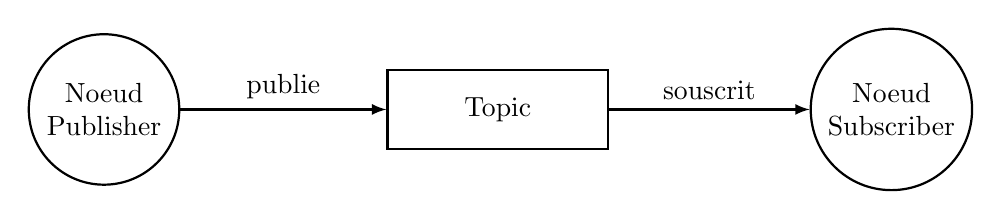
\begin{tikzpicture}[>=latex]
        % Styles
        \tikzstyle{rosnode}=[circle, draw, thick, minimum size=14mm, align=center]
        \tikzstyle{topic}=[rectangle, draw, thick, minimum width=28mm, minimum height=10mm, align=center]

        % Nodes
        \node[rosnode] (pub) at (0,0) {Noeud\\Publisher};
        \node[topic]   (top) at (5,0) {Topic};
        \node[rosnode] (sub) at (10,0) {Noeud\\Subscriber};

        % Arrows
        \draw[->, thick] (pub) -- node[above]{publie} (top);
        \draw[->, thick] (top) -- node[above]{souscrit} (sub);
    \end{tikzpicture}
    \caption{Schéma ROS~2 publisher-subscriber via un topic}
    \label{fig:ros2_topic}
\end{figure}

En 2017, une nouvelle version majeure de \gls{ros} a été publiée, appelée \gls{ros2} \cite{noauthor_distributions_nodate}. Elle a apporté plusieurs améliorations par rapport à \gls{ros1}. Avec la première version, il était nécessaire de définir un \textit{master} centralisé pour gérer la communication entre les noeuds, ce qui limitait la scalabilité et la robustesse du système. A l'opposé, \gls{ros2} utilise le protocole \gls{dds} pour la communication entre les noeuds, ce qui permet une architecture décentralisée et plus flexible; il n'y a plus besoin de déclarer un \textit{master}. De plus, \gls{ros2} offre un meilleur support pour les systèmes temps réel, une meilleure gestion des ressources (mutli-threading) et une meilleure compatibilité avec les différents systèmes d'exploitation (Windows, Linux et MacOS). 
\gls{ros2} est compatible avec les systèmes embarqués, grâce à la librairie Micro-ROS, qui permet d'exécuter des noeuds \gls{ros2} sur des microcontrôleurs aux ressources limitées comme par exemple une carte Arduino. 
Aussi, \gls{ros1} n'est a ce jour plu maintenu et mis à jour, c'est pourquoi \gls{ros2} a été choisi pour le développement des programmes de contrôle des robots durant ce projet.

